\section{Conception}

\subsection{Introduction}
\begin{prettyBox}{Conception Introduction}{mypur}
Conception represents the solution to a problem, expressed through structured diagrams such as UML.
Creating a conception is an iterative process that requires significant time and creativity.
Initially, a solution is developed, and subsequent iterations focus on optimizing it.

\vspace{0.15cm}
Each iteration refines and expands the conception until reaching a final result that is easy to
maintain. This ensures better implementation, facilitates adding or removing features, and 
simplifies bug fixes.

\end{prettyBox}

\vspace{0.5cm}
\begin{prettyBox}{Difference Between Conception \& UML}{red} 
    \begin{center} 
        \textbf{Conception $\not\Leftrightarrow$ UML} 
     \end{center}
UML is merely a tool used to represent the conception, it is not the conception itself. 
Conception encompasses more than just diagrams—it includes algorithms, explanations of 
diagrams, and other documents.
\end{prettyBox}


\vspace{0.5cm}
\begin{prettyBox}{Importance of Maintainability}{red} 
Easy maintainability is one of the key qualities of a good conception and arguably the most
important criteria. This is because we want the software to be long-lasting, and effective 
maintenance is essential to achieving that.
\end{prettyBox}

\vspace{0.5cm}
\subsection{Itterative Process Of Conception}

\begin{prettyBox}{Global \& Detailed Conception}{mypur}
    \begin{itemize}
        \item \textbf{Globale Conception :} Modules must be identified (some modules can 
be divided into sub-modules) , and interaction between modules must be defined
        \item \textbf{Detailed Conception :} Each module must be defined independently in detail.
    \end{itemize}
The conception should have high ratio of cohesion and low ratio of coupling
\end{prettyBox}

\vspace{0.5cm}

\begin{prettyBox}{Why Global Conception Then Detailed Conception}{red} 
    We first define the high-level structure of the modules and their interactions to provide an overall system architecture.
    This gives a clear overview of the software before delving into the detailed characteristics of each module.
\end{prettyBox}

\vspace{0.5cm}


\begin{prettyBox}{Why High Cohesion \& Low Coupling}{red}
    \begin{itemize}
        \item \textbf{Cohesion}: How related the responsibilities of a module are.
            \begin{itemize}
                \item \textbf{High Cohesion}: The module has a clear, well-defined responsibility, making it easier to understand, maintain, and modify.
                \item \textbf{Low Cohesion}: The module handles multiple, unrelated responsibilities, making it harder to maintain and understand.
            \end{itemize}
        \item \textbf{Coupling}: How dependent the modules are on each other.
            \begin{itemize}
                \item \textbf{High Coupling}: Modules are highly dependent on each other. A failure in one critical module may cause the entire system to fail.
                \item \textbf{Low Coupling}: Modules are loosely connected, and changes or failures in one module are less likely to impact the others.
            \end{itemize}
    \end{itemize}
    
    \textbf{Why We Want High Cohesion and Low Coupling}:
    \begin{itemize}
        \item \textbf{High Cohesion}: Ensures that each module has a clear, understandable purpose, making the system easier to maintain and extend.
        \item \textbf{Low Coupling}: Reduces dependencies between modules, minimizing the risk of widespread system failure and increasing flexibility.
    \end{itemize}
\end{prettyBox}


\vspace{0.5cm}

\subsection{Classification Of Conception Method}

\vspace{0.25cm}
\subsubsection{Function Oriented Conception}

\vspace{0.25cm}
\begin{prettyBox}{Function-Oriented}{mypur}
    The software is structured using a functional paradigm. It is divided into a set of functions 
that interact with each other. The software is viewed as a complex main function that is 
progressively decomposed into smaller, less complex sub-functions. This process continues until
we reach a detailed conception.

    \vspace{0.15cm}
    Each function has its own local state (local variables), while the software has
a global state (global variables) that is shared among all functions.
\end{prettyBox}

\vspace{0.5cm}
\subsubsection{Object Oriented Conception}

\vspace{0.25cm}

\begin{prettyBox}{Object-Oriented Design}{mypur}
    The software is viewed as a collection of encapsulated and independent objects. 
These objects communicate with each other by sending messages (method calls).

    \vspace{0.15cm}
    Each object is identified by its name and encapsulated attributes (variables and methods).
\end{prettyBox}


\vspace{0.5cm}

\subsubsection{Data Oriented Conception}

\vspace{0.25cm}

\begin{prettyBox}{Data-Oriented}{mypur}
    The software's structure must reflect the structure of the data it traits .
    Therefore the conception is influenced by the ouput input data.
\end{prettyBox}


\subsection*{\underline{Example :}}
Compiler

\vspace{1cm}

\subsection{Conception's Principales}To make sure the conception ensures an easily maintainable
software we must follow some printcipales :


\begin{prettyBox}{Principles}{mypur}

\begin{itemize}
    \item \textbf{Abstraction:} Focuses on the essential characteristics while
hiding unnecessary details.
    \item \textbf{Modularity:} Divides the system into modules with well-defined interactions,
adhering to the principle of high cohesion and low coupling.
    \item \textbf{Encapsulation:} Hides internal details of a module from other modules.
    \item \textbf{Structuring:} Ensures a structured conceptions (levels) , we can at least have general \& detailed conception.
\end{itemize}

\end{prettyBox}

\vspace{0.5cm}

\subsection{Notation For Fonctional Conception}


\begin{prettyBox}{Notation}{mypur}
\begin{itemize}
    \item \textbf{Data Flow Diagram (DFD):} Shows how data is transformed and passed from one module to another.
    \item \textbf{Structure Diagram (SD):} A hierarchical diagram that illustrates the structured relationships between the components of the software.
\end{itemize}
\end{prettyBox}


\vspace{0.5cm}

\begin{prettyBox}{Relation Between DFD \& SD}{red}
    DFD and SD are complementary to each other, working together to clearly describe the functional design of a software system.
\end{prettyBox}

\vspace{0.5cm}

\subsubsection{DFD}

\vspace{0.25cm}

\begin{prettyBox}{DFD}{mypur}
    A DFD diagram consists of four components:
    \begin{itemize}
        \item \textbf{Transformations}: Represented as circles.
        \item \textbf{Data}: Represented as axis.
        \item \textbf{Logical AND}: Represented by the symbol *.
        \item \textbf{Logical OR}: Represented by the symbol +.
    \end{itemize}
\end{prettyBox}

\vspace{0.5cm}

\begin{center}
    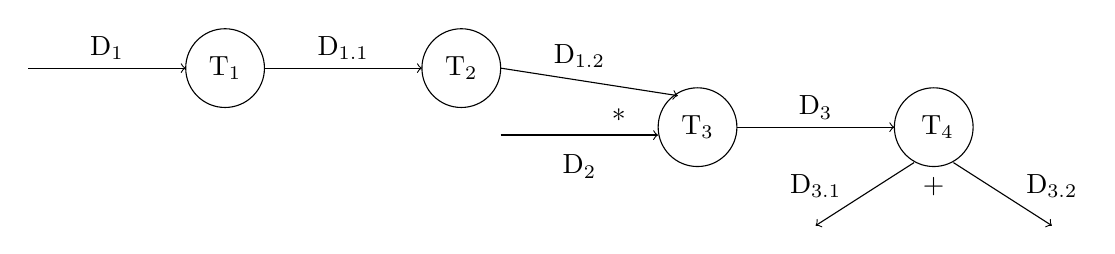
\begin{tikzpicture}
        \draw[->] (0,0) -- (2,0);
        \node at (1,0.25){D$_{1}$};
        \draw (2.5,0) circle (0.5);
        \node at (2.5,0) {T$_{1}$};
        
        \draw[->] (3,0) -- (5,0);
        \node at (4,0.25){D$_{1.1}$};
        \draw (5.5,0) circle (0.5);
        \node at (5.5,0) {T$_{2}$};

        \draw[->] (6,0) -- (8.25,-0.35);
        \node at (7,0.15){D$_{1.2}$};
        \draw (8.5,-0.75) circle (0.5);
        \node at (8.5,-0.75) {T$_{3}$};
        
        \draw[->] (6,-0.85) -- (8,-0.85);
        \draw[->] (9,-0.75) -- (11,-0.75);
        \node at (7.5,-0.65) {*};
        \node at (7,-1.25) {D$_{2}$};
        \node at (10,-0.5) {D$_{3}$};
        \draw (11.5,-0.75) circle (0.5);
        \node at (11.55,-0.75) {T$_{4}$};
        \draw[->] (11.25,-1.2) -- (10,-2);

        \node at (11.5,-1.5) {+};
        \draw[->] (11.75,-1.2) -- (13,-2);

        \node at (13,-1.5) {D$_{3.2}$};

        \node at (10,-1.5) {D$_{3.1}$};

    \end{tikzpicture}
\end{center}

\vspace{0.5cm}

\begin{prettyBox}{Note}{red}
    A DFD specifies the operations without detailing how they are performed. Each node in the diagram can be further described with another DFD, allowing for a hierarchical decomposition of processes.
\end{prettyBox}

\vspace{0.5cm}

\subsection*{\underline{Example :}}
A Software that processes a text document by splitting it into individual
words. It then checks each word against a dictionary. If the word exists in
the dictionary, it is marked as correct. Otherwise, the software notifies the
user and allows them to decide whether the word is valid. If the user 
identifies the word as incorrect, it is added to the list of misspelled words.
If the user confirms the word is valid, it is added to the dictionary.

\begin{center}
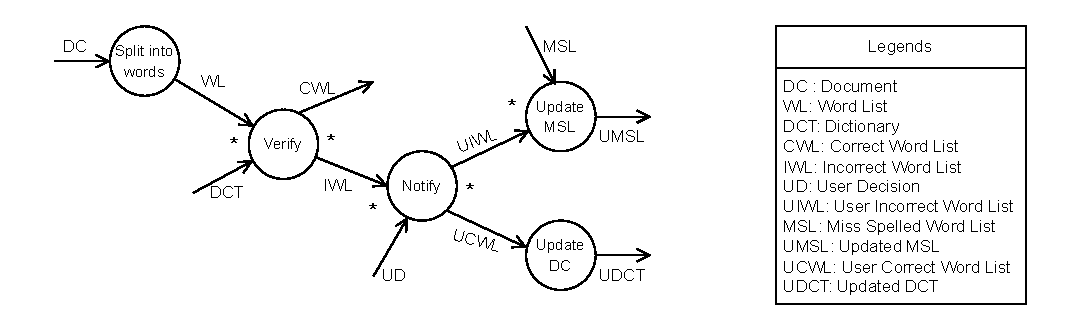
\includegraphics[width=0.9\textwidth]{Chapters/Diagram/DFD/dfd2.drawio.pdf}
\end{center}

\subsubsection{SD}

\begin{prettyBox}{SD}{mypur}
A structure diagram is a hierarchical representation of a system in the
form of a tree. It illustrates how the transformation elements of a Data Flow
Diagram (DFD) can be implemented within the hierarchical units of software architecture.
\end{prettyBox}

\vspace{0.25cm}

\begin{prettyBox}{Difference Between SD \& DFD}{red}
They might seem similar but they serve different purposes and compliment each other ,
SD shows how the data changes and flows with the transformation , and DFD focuses on the hiertachy
of the software architecture
\end{prettyBox}

\subsubsection*{Symboles}

\begin{center}
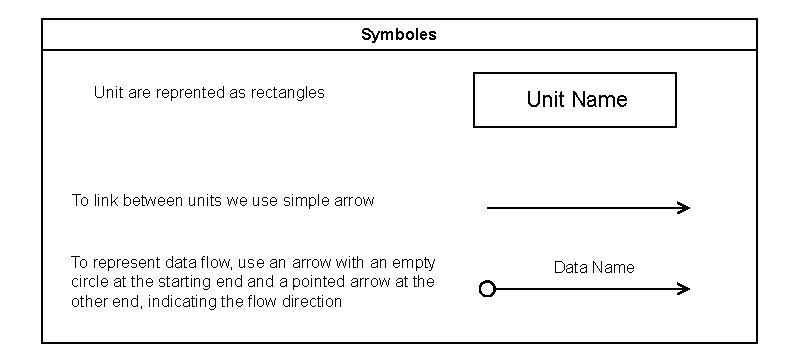
\includegraphics[width=0.9\textwidth]{Chapters/Diagram/SD/smb.drawio.pdf}
\end{center}

\vspace{0.5cm}

\subsubsection*{Tree Nodes}
\begin{itemize}
    \item \textbf{Synchronisation Unit} : The root node at the top represent the the global idea of the software 
    \item \textbf{Transformation Unit} : The parent node has to point to at least one other units , represent a function of the software
    \item \textbf{Input/Output Unit} : The leaf node same as parent node just never points to another unit
\end{itemize}

\vspace{0.5cm}

\begin{prettyBox}{Note}{red}
\textbf{\underline{Synchronisation Unit's Role}}\\[0.15cm]
The synchronisation unit (root node) never creates the data it only pass it to other units.\\[0.25cm]
\textbf{\underline{No Link Between Unit Of Same Level}}\\[0.15cm]
There can be link between units with simple arrow only with units of different level.\\[0.25cm]
\textbf{\underline{SD Level}}\\[0.15cm]
It's the number of levels beside the root node (don't count the synchronisation unit).
\end{prettyBox}

\begin{center}
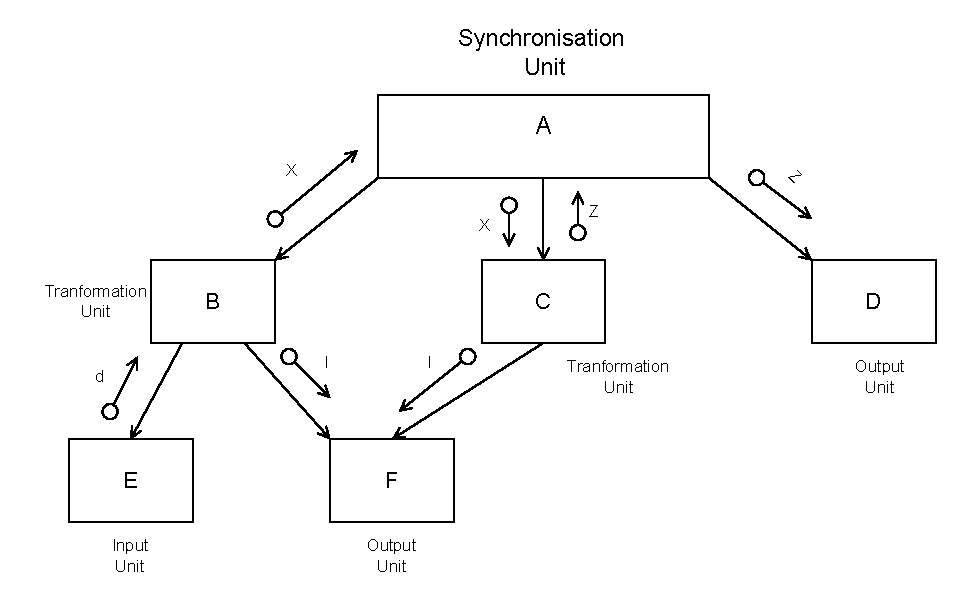
\includegraphics[width=0.85\textwidth]{Chapters/Diagram/SD/sd1.drawio.pdf}
\end{center}

\vspace{0.25cm}

\subsection*{\underline{Example :}}
We will take same example of word checker, we will make level 1 SD then level 2 SD

\subsection*{\underline{Level 1 SD :}}
\begin{center}
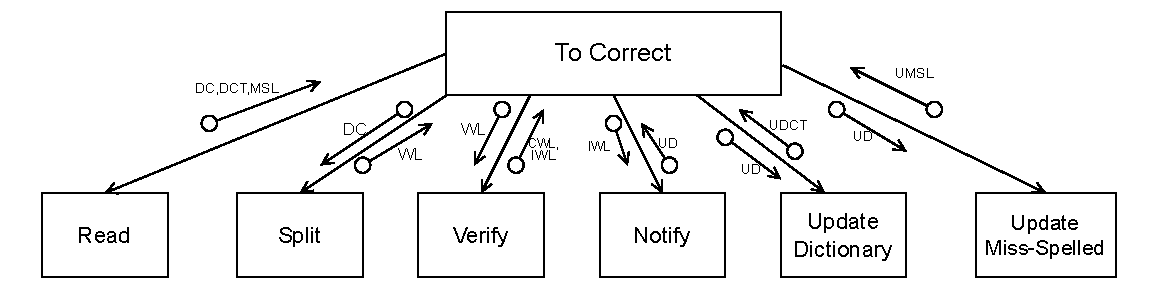
\includegraphics[width=0.85\textwidth]{Chapters/Diagram/SD/sd2.drawio.pdf}
\end{center}



\subsection*{\underline{Level 2 SD :}}
\begin{center}
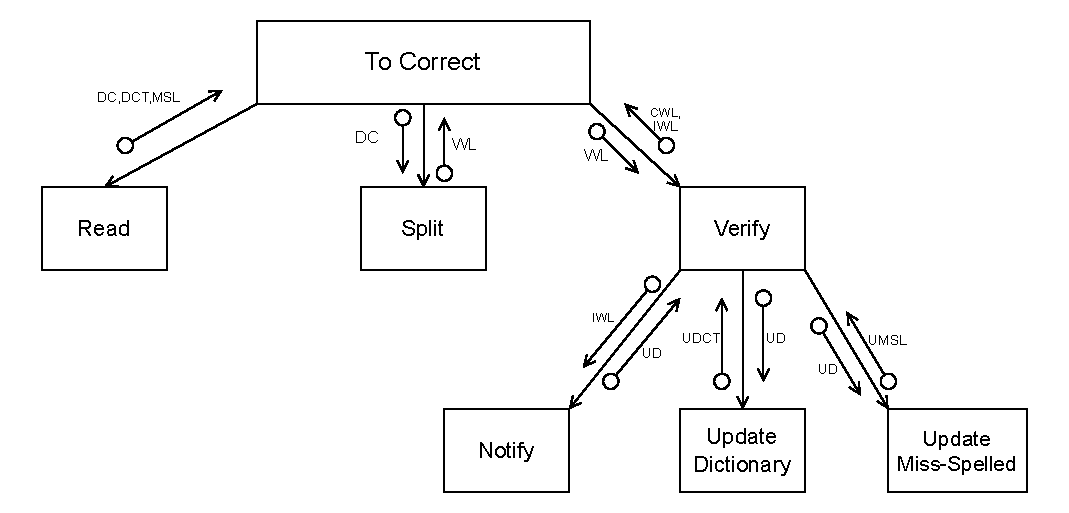
\includegraphics[width=0.8\textwidth]{Chapters/Diagram/SD/sd3.drawio.pdf}
\end{center}

\vspace{1cm}
\subsubsection{Sequence Diagram}


\begin{prettyBox}{Sequence Diagram}{mypur}
A sequence diagram illustrates the dynamic behavior of a system over time (notion of time). 
It visualizes the messages exchanged between objects/actors and is read from top to bottom.
\end{prettyBox}

\subsection*{\underline{Symboles :}}

\begin{center}
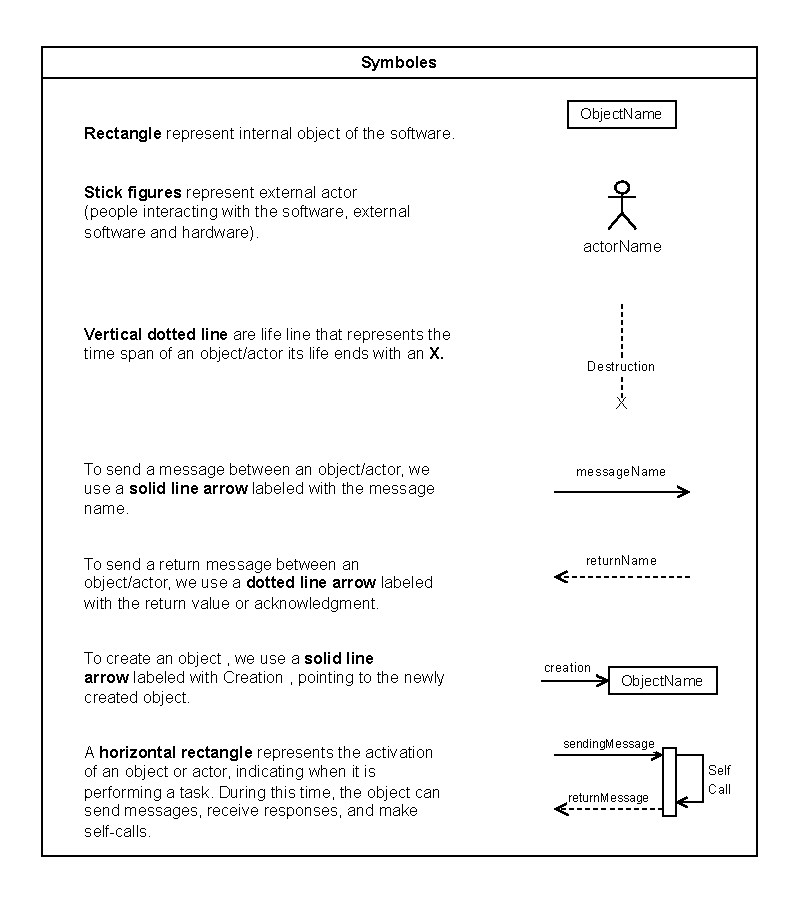
\includegraphics[width=0.8\textwidth]{Chapters/Diagram/SQD/sym.drawio.pdf}
\end{center}


\subsection*{\underline{Example :}}

\vspace{0.25cm}
\begin{center}
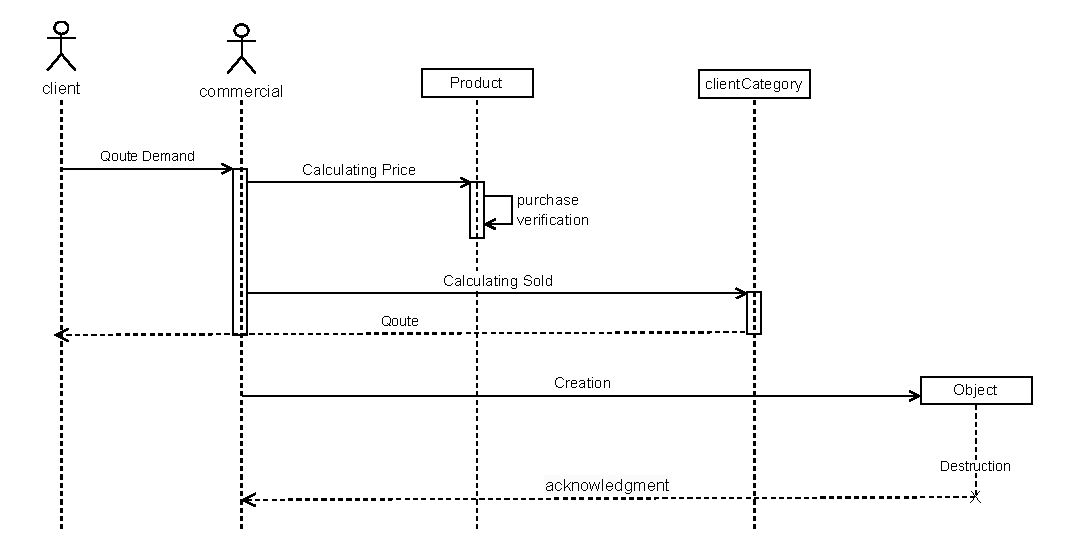
\includegraphics[width=0.95\textwidth]{Chapters/Diagram/SQD/sqd.drawio.pdf}
\end{center}


\vspace{1cm}
\subsubsection{State-Transition Diagram}

\begin{prettyBox}{State Diagram}{mypur}
A state diagram illustrates how the state of an object changes in response to events.
\end{prettyBox}

\subsection*{\underline{Symboles :}}

\begin{center}
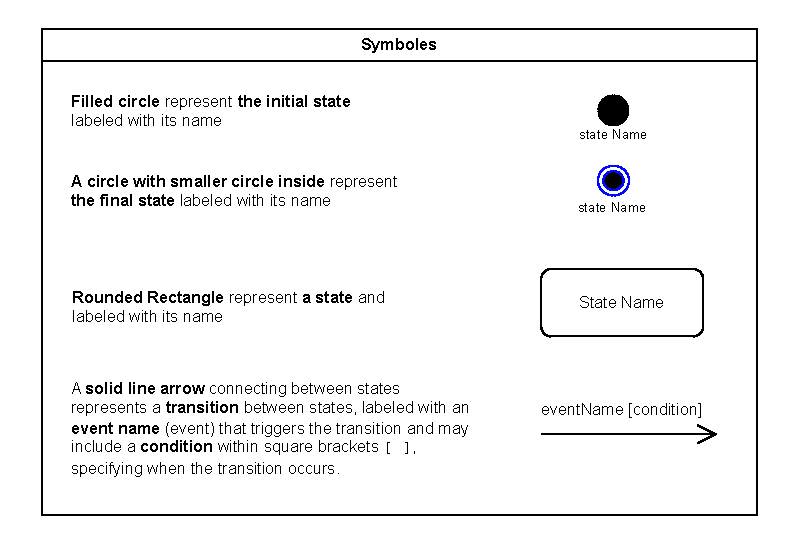
\includegraphics[width=0.8\textwidth]{Chapters/Diagram/ST/sym.drawio.pdf}
\end{center}

\vspace{0.25cm}

\begin{prettyBox}{Note}{red}
We can have only \textbf{one initial state} , but we can have \textbf{many final state}.
\end{prettyBox}

\subsection*{\underline{Example :}}

\begin{center}
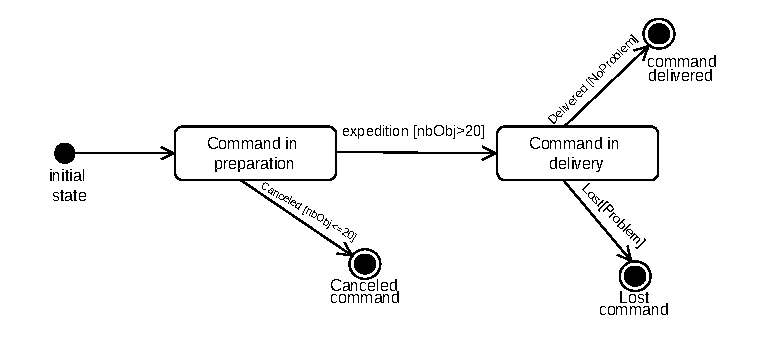
\includegraphics[width=0.95\textwidth]{Chapters/Diagram/ST/state.drawio.pdf}
\end{center}


\vspace{1cm}
\subsubsection{Activity Diagram}

\begin{prettyBox}{Activity Diagram}{mypur}
An activity diagram describes the progression of activities within the system and outlines the logical flow of processes.
\end{prettyBox}

\subsection*{\underline{Symboles :}}

\begin{center}
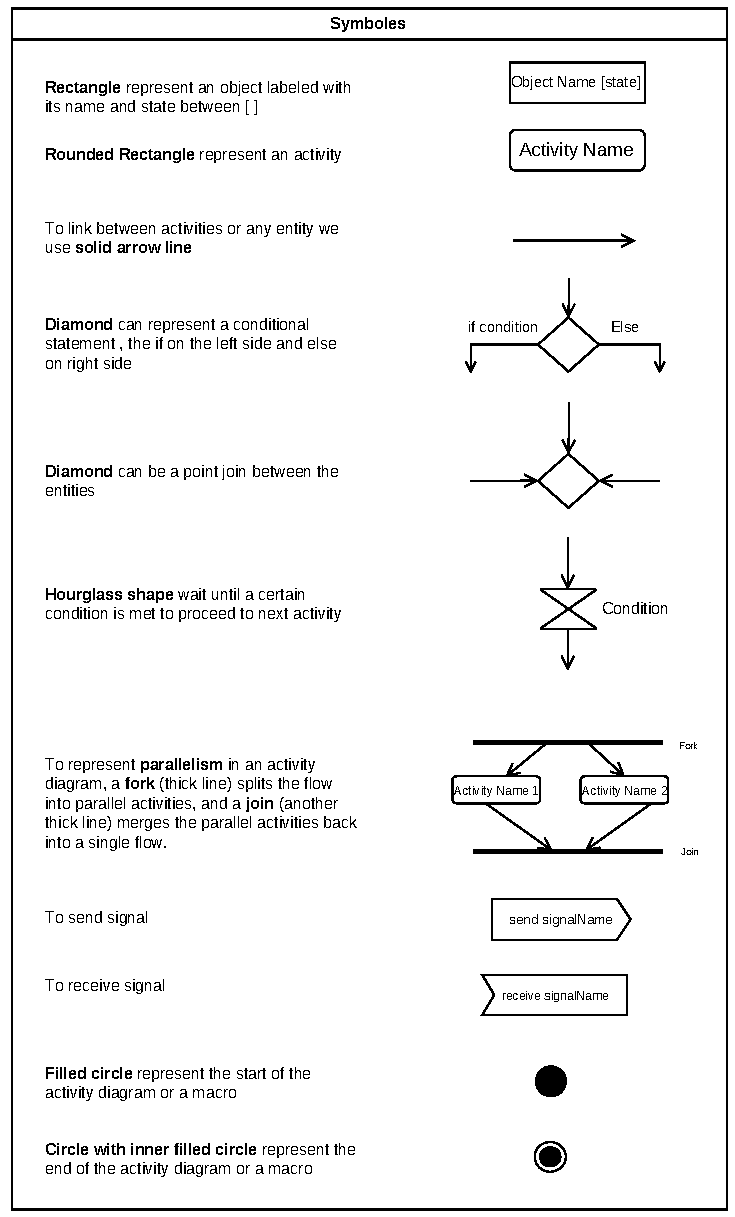
\includegraphics[width=0.85\textwidth,height=0.97\textheight]{Chapters/Diagram/AC/sym.drawio.pdf}
\end{center}


\subsection*{\underline{Example :}}


\begin{center}
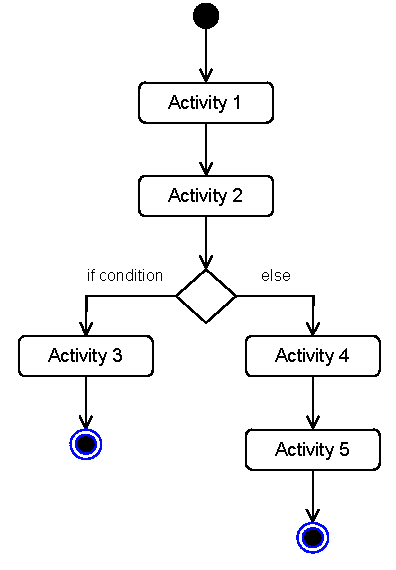
\includegraphics[width=0.7\textwidth,height=0.8\textheight]{Chapters/Diagram/AC/ac1.drawio.pdf}
\end{center}

\begin{center}
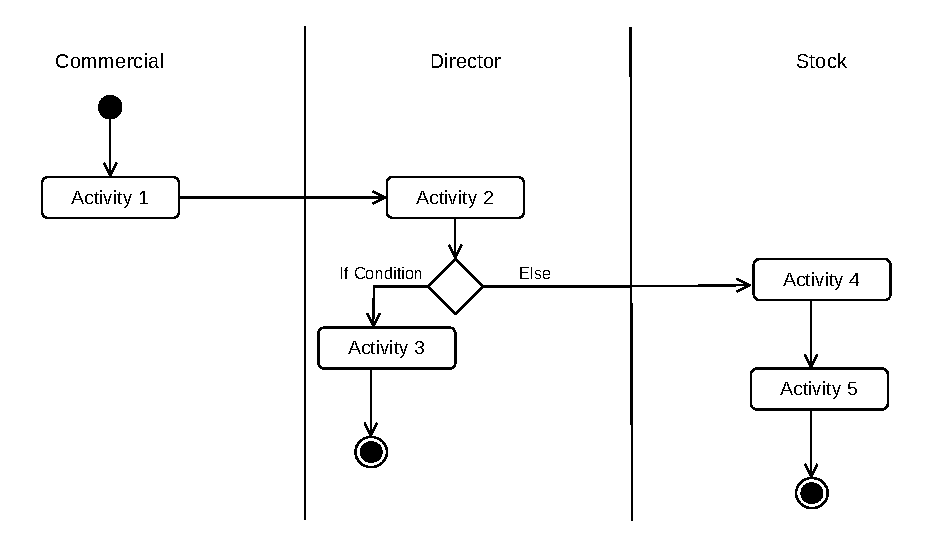
\includegraphics[width=0.9\textwidth,height=0.78\textheight]{Chapters/Diagram/AC/ac2.drawio.pdf}
\end{center}



\vspace{0.25cm}

\begin{prettyBox}{Note}{red}
\begin{itemize}
    \item We can have only \textbf{one begin} , but we can have \textbf{end}.
    \item Even though activity diagram has the notion of state it focuses more on the 
    logical flow of activities of the system.
\end{itemize}
\end{prettyBox}



